\section{Introduction}

Android allows developers to write native code that is able to interact with the Java code. This can be accomplished with the Native Development Kit (NDK). The NDK documentation declares the Native Development Kit useful in the following cases \cite{AndroidNdkIntro}:

\begin{itemize}
	\item Squeeze extra performance out of a device to achieve low latency or run computationally intensive applications, such as games or physics simulations.
	\item Reuse your own or other developers' C or C++ libraries. 
\end{itemize}

In \cite{5669738} was shown that the use of native code can considerably speed up Java applications.

As stated in \cite{AndroidNdkIntro} , the communication between Java and the native code is done via Java Native Interfaces(JNI) \footnote{\url{https://docs.oracle.com/javase/8/docs/technotes/guides/jni/spec/jniTOC.html}}. 
JNI is a native programing interface, so that Java code running in the JVM can interoperate with applications and libraries written in other programming languages \cite{JNISpecChapter1}.

JNI wasn't designed with security in mind and doesn't do any security checks. This fact can be derived from the design specification document from JNI (section 'Reporting Programming Errors')\cite{JNISpecChapter2}.
The native code has direct access to the memory of the running process and
since the Java and native code are running in the same memory address space, the native code is able to read and write arbitrary memory from the JVM \cite[p. 2]{Afonso2016GoingNU}.

In sum is to register, that JNI is a powerful tool without
restricting the developer. Speeding up execution
of native code is convenient for developers, yet, from a security perspective it is also a very dangerous tool. If an attacker is able to execute code in a native library the executed code can also abuse the power of JNI.\\

A selection of possible attacks exploiting JNI are:
\begin{itemize}
\item As native libraries reside in the same address space as a JVM, bugs in native
libraries can enable attackers to read and write the JVM's memory \cite[p. 3]{Sun_jvm-portablesandboxing}. %\textbf{TODO:} Mention example attack
	\item  Similar to the Reflection API, JNI allows to retrieve and set the content of private fields. This enables an attacker to steal confidential information \cite[p. 3]{Sun_jvm-portablesandboxing}.
	\item JNI allows to set the destination of an object pointer without type-checking. Thus type-confusion attacks are possible \cite[p. 4]{Sun_jvm-portablesandboxing}. %\textbf{TODO:} What can be achieved by type confusion attacks?
	\item Bugs in the Linux kernel can enable an attacker to escalate privileges, like done in 'Dirty Cow' (CVE--2016--5195) \cite{DirtyCow}. Over JNI such attacks can directly be initiated
    \item Changing the behavior of the Java application by replacing functions by manipulating or injecting byte code using code patching methods.
	\item Changing the behavior of the Java application by replacing functions by manipulating or injecting byte code using code patching methods.
	We will present later in this paper an example for this kind of attack.
\end{itemize}


There is to be emphasized that quite a few Android apps use native code: A survey of Google Play apps \cite[p. 3]{Sun:2014:NPA:2627393.2627396} revealed, that 86\% of the top 50 apps have been shipped with native code. There were also apps (like Skype), that use native code for a common core being shared among multiple platforms. If an app would be compromised through a flaw in the native code, possible thousands or even millions of systems would be affected and these apps could be an interesting target for attackers.\\


In this paper we will analyze how the security vulnerabilities exposed by JNI can be abused by an attacker, if he is able to execute code in a native library, and how the attacker can compromise the benign target app using native code.
The following sections of this paper are structured as follows: 
\begin{itemize}
\item In Section 2 we will look at other works dealing with
security concerns of native code
\item In Section 3 we will discuss techniques and methods as working basis for Section 4
\item In Section 4 finally the aforementioned attack scenario will be presented
\end{itemize}


\section{Related work}
YAHFA is a framework, that allows to hook arbitrary java methods and redirect the execution to another java method \cite{YahfaGithub}. We used YAHFA as a reference project for implementing our attack. 
 
Until 2014, the security threats coming from native libraries wasn't given that much attention. Mistakenly it was assumed that native code would be as secure as Java code since Android regulates all components above the kernel \cite[p. 1]{Sun:2014:NPA:2627393.2627396}.
But in recent years, more effort was done in finding ways to make native library calls more secure.

In \cite{Afonso2016GoingNU} the authors analyzed dynamically about of 446 thousand Android apps that use native code and developed a Native-Code policy that limits many malicious behaviours while still allowing the correct execution of 99.77\% of the benign apps.

The authors from \cite{Sun:2014:NPA:2627393.2627396} present a security framework called NativeGuard, that isolates and executes code from native libraries in a separated non-privileged application. The communication with the source app is done via interprocess communication. Through NativeGuard native libraries don’t inherit privileges from the Android app and cannot access anymore the memory from it.
Also a well known software sandboxing project is Robusta \cite{Siefers:2010:RTN:1866307.1866331}. %\textbf{TODO: More Description}

Not explicitly designed for Android, but nevertheless an interesting project is CHERI JNI, that is a hardware-assisted implementation of JNI extending the guarantees required for Java's security model to native code \cite{Chisnall:2017:CJS:3093337.3037725}.

In \cite{ExecuteThis} the security implications of loading additional code from external sources at runtime have been analyzed. Attackers can abuse the code loading to hide malicious code from security services like Google Bouncer. But benign applications can also have vulnerabilities, if the code loading is done insecurely. It was found out, that Android doesn't enforce enough security checks on external code and developers of benign apps often don't implement right appropriate protection mechanisms or are unwitting of the threats. The authors have done a large-scale analysis of popular Google Play apps and have laid bare that 9.25\% of them are vulnerable to code injection attacks. As a sample attack they did a HTTP Man-In-The-Middle attack (MITM) on a benign application:
They exploited an insecure http connection. The stated app had implemented an update process where the update was downloaded from a remote HTTP server. The update is then loaded through a Classloader at runtime. But by using the insecure HTTP connection instead of HTTPS, the application is vulnerable to a MITM attack, through which again an attacker could execute arbitrary code that is allegedly considered to be an update.
With the results of the analysis they modified the Dalvik VM in such a way that attacks through external code loading can be blocked. They did this by adding missing security checks for external sources.\\

Most of the apps out there are free apps, as shown in \cite[p. 164]{Wang:2017:ESM:3038912.3052712}, that 15\% of all Android apps are paid apps, however they only account for 0.2\% of the total app installs. 
Thus, it is not surprising that the developers of free apps like to use advertising libraries: 

A survey of 2012 showed that 49\% of all apps and 50\% of the top free apps used libraries for monetarized advertising \cite[p.7]{Pearce:2012:APS:2414456.2414498}. 
Advertising libraries have a large user base and thus security plays even a major role. 
If an advertising library gets compromised through a malicious insider or a flaw in the native code, this could guide to fatal consequences. 
An actually well-intentioned C code could lead through memory safety vulnerabilities to arbitrary code injection as elaborated in \cite{Szekeres:2013:SEW:2497621.2498101}.

\section{Background}

In this section we look at some background knowledge, necessary for understanding the attack scenario, which will be presented in the following section.
 
\subsection{Java Native Interface}

Loading a native library from Java can be accomplished by:
\begin{lstlisting}[language=Java, style=JavaCodeStyle, caption=Loading a native libary]
 System.loadLibrary("libName");
\end{lstlisting}
Where \emph{libName} is the name of the native library without file extension since the file extension is platform dependent.

The declaration of a native method is done in Java as well. It resembles the declaration of an interface method, but uses the 'native' keyword:
\begin{lstlisting}[language=Java, style=JavaCodeStyle, caption= native declaration]
package com.example;
public class Native {
  public native String fromNative();
}
\end{lstlisting}

The definition of  a native method is done using native code (here C++). This example defines a native method, that returns a \emph{java.lang.String} class object.
\begin{lstlisting}[language=C++, style=CppCodeStyle, caption=Native Hello World Example]
extern "C" JNIEXPORT jstring JNICALL
Java_com_example_fromNative(JNIEnv *env,jobject /* this */) {
    const char* msg = "Hello from C++";
    return env->NewStringUTF(msg);
}
\end{lstlisting}

Over the JNIEnv variable \emph{env}, the C programer can access the methods of the JNI interface. The JNIEnv variable is created by the JVM. Before the native function is called, a pointer to the JNIEnv variable is pushed on the callstack as the first parameter. The second argument of type jobject is a pointer to the java object the native method is called from. For static native methods, a pointer to the class the native method belongs to, is pushed instead. 

\subsection{Android Runtime (ART)}
In Android, currently there exist two Virtual machines: The older solely JIT-compiling Dalvik and the newer one: ART. ART introduced Ahead-of-time compilation (AOT) in Android \cite{ArtAndDalvik}. AOT precompiles the majority of the java code on install time, which speeds up program starts of apps. ART replaced Dalvik in Android 5.0 (Lollipop) \footnote{\url{https://developer.android.com/about/versions/android-5.0-changes.html}}. For that reason, we will design our attack scenario exploiting ART internals, as Dalvik isn't used anymore in newer Android versions. But it should be noted, that a similar attack would be possible for the Dalvik runtime.

In Android 7.0 (Nougat) a JIT Compiler was again reintroduced that works along with the AOT compiler \cite{Android7ForDevelopers}. The reason for this were to improve runtime performance, saving storage space and speeding up application and system updates \cite{JitWorkFlow}.

On a simplified view, the new JIT-Compiler basically works like follows:  


\begin{itemize}
    \item Only 'hot' methods are compiled Ahead-of-time 
    \item A method is 'hot' if it is called often.
    \item On install time an analyzing process decides which methods are likely to be 'hot'.
    \item On runtime, the Analyzer checks regularly if a method is 'hot'
    \item If a method gets 'hot', it will be compiled by the AOT compiler
    %\textcolor{red}{TODO: Move to attack scenario}
    %$\Rightarrow$ In order to replace an existing java method, the method has to be set to native and its 'hotness' count has to be set to 0 (not 'hot')
    \end{itemize}
    
In figure \ref{JitWorkflow} we see how the new JIT compilation works starting from Android 7.0.     
    
\begin{figure}[H]
	\begin{center}
	%\vspace*{-0.1cm}
		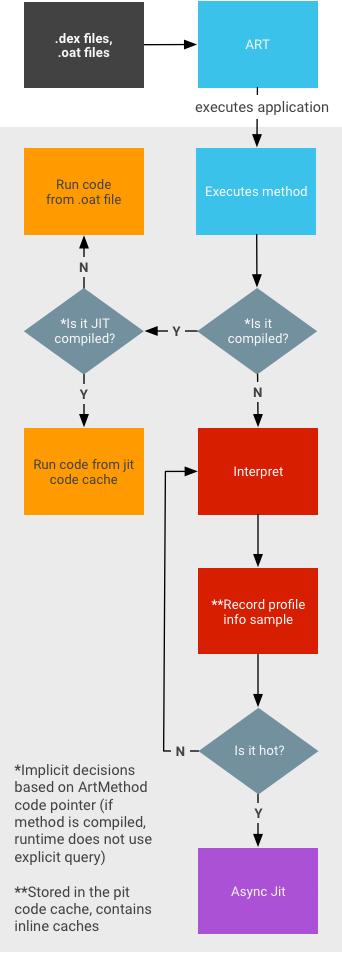
\includegraphics[scale=0.45]{figures/jit-workflow-extract.png}
	\end{center}
	\caption{Extract from the JIT Workflow on Android 7.0 and above \cite{JitWorkFlow}}
	\label{JitWorkflow}
\end{figure}

When compiling an android app, the Java source files get compiled first to *.class files as usual and then compiled to Dalivk bytecode. The resulting code is stored into a  Dalvik Executable (DEX) file and finally packed into an Android Package Kit (APK). This process is independent from the VM used by the target android device.

Now we assume on the target device is installed Android 7.0 or above.
While installing the app, ART analyzes the *.dex files and optimizes the code. As a result of this optimization step, 'hot' methods get AOT compiled and stored in *.oat files, that are binary files for AOT compiled methods.


When an Android app starts, the corresponding *.dex and *.oat files get loaded to memory by ART. The JIT-compiler checks upon the calling of a method, whether the method is compiled or not. If the method is compiled, it is further checked, whether the compiled method is AOT-compiled or JIT-compiled. The result of the checks determines, whether the method is run from the *.oat file or from the JIT code cache.

Should the method to be executed not be a compiled method, the method goes through several steps: At first it is executed by the interpreter, than a profile sample is recorded and as the last step it is checked, whether the method is 'hot'. If the method is not 'hot', its hotness counter is incremented. 
If the method is 'hot' the method is (asynchronously) JIT compiled.

From the JIT workflow we can note that a native function will never be 'hot' or JIT-compiled as it is considered to be compiled. That conclusion may sound trivial but it will play a central role later in the attack scenario. 

\subsection{ART Internals}

In this section we analyze how a java method is stored in memory and how the method is processed by ART when the method gets called by user code. As the internals of ART can change from revision to revision (so very frequently), we concentrate on Android 8.0 rev. 36, which is the release version of Android 8 (Oreo). This is also the android version our attack scenario is targeting at.

When loading an app, ART creates for each java method an ArtMethod object. The ArtMethod class is used to store runtime information for each java method. For example, it is stored if the method is public, private or protected, in which class it is defined, whether it is synchronized or native, etc. . 
In listing \ref{ArtMethodLabel} we see the definition of the ArtMethod class like it is defined in Android 8 rev. 36:

\begin{lstlisting}[language=C++, style=CppCodeStyle, caption=ArtMethod and x86 offsets \cite{ArtMethodOreoRev36}, label=ArtMethodLabel,
escapechar=!]
class ArtMethod FINAL { 
 protected:
  GcRoot<mirror::Class> declaring_class_;// 0
 !\colorbox{yellow}{std::atomic<std::uint32\_t> access\_flags\_;}! // 4
  uint32_t dex_code_item_offset_; // 8
  uint32_t dex_method_index_; // 12
  uint16_t method_index_; // 16
  !\colorbox{yellow}{uint16\_t hotness\_count\_;}! // 18
  struct PtrSizedFields {
    ArtMethod** dex_cache_resolved_methods_; // 20
    !\colorbox{yellow}{void* data\_;}! // 24
    !\colorbox{yellow}{void* entry\_point\_from\_quick\_compiled\_code\_;}! // 28
  } ptr_sized_fields_;
};
\end{lstlisting}

The listing contains the definition of the ArtMethod and x86 class offsets (measured in bytes). The offsets define the memory layout for the x86 architecture. For now we can just ignore the offsets since we will need them only for the attack implementation.

We won't go into all details, but we discuss the yellow highlighted class members as they are a help for our attack:

\begin{itemize}
\item \textbf{access\_flags\_}: Is a bitwise flag field. Is used to specify the visibility of the method (public, protected, private), whether the method is synchronized and similar stuff. There exists also a native flag, that marks the method as native.
\item \textbf{hotness\_count\_}: Counter for tracking how often the java method has been called. Is used to determine if a java method is 'hot'. It is not used if the java method is native.
\item \textbf{data\_}: Is used for several purposes, but if the java method is native, it always points to the native code.
\item \textbf{entry\_point\_from\_quick\_compiled\_code\_}: points to machine code that has to be executed before the actual java method is called. So that machine code functions as a \emph{prolog}. Independent from the type of java method, the prolog always is called.
\end{itemize}

\subsection{Function Hooking}
Function hooking means to intercept the call of a function and redirect the execution flow to another memory address.
For machine code, this is done by writing a jump or return instruction to the beginning of the function to be hooked. This way one can jump/redirect the execution flow to a custom code location. 
Whenever the hooked function gets called, now the custom code (which we now call \emph{hook function}) is called.

But there arises a problem now: What if we want to call the original function from inside the hook function? When applying the hook, the first instruction of the hooked function get destroyed. So, one has to do somehow a backup of the original function before hooking it. This process of doing a backup and than applying a function hook, is called \emph{trampoline} hook and is coined by Microsoft's Win32 API hooking library Detour \cite{detours-binary-interception-of-win32-functions}.

As java methods aren't directly laid out as machine code instruction, doing a trampoline hook on an android app works a bit differently. There might be more ways to do it, but we will discuss the way it is done in the YAHFA Hooking Library \cite{YahfaGithub}:\\

As a first step, the java method, that should be hooked, is made a native method. This can be done by assigning the corresponding ArtMethod the native flag to the access\_flags\_ field. Different types of java methods (e.g. native methods, JIT-compiled or OAT compiled) are handled differently by ART. By making the method native, we don't need to differentiate between the different types of java methods.\\

The second step is to assign the \\\emph{entry\_point\_from\_quick\_compiled\_code\_} field to a memory address where user defined code lies. In YAHFA this is dynamically created code that will redirect to another java method (the hook method). In our attack we will also do this. In the implementation section we will discuss why we did it this way.

In order to call the original java method, before any changes are performed all class members that are going to be changed are stored in a backup. 
Therefore the original (hooked) java method is copied and its content is stored in a new java method (the so-called bakup method).
But there are two things to consider:

First, the backup method mustn't be JIT-compiled, otherwise the set hook will be destroyed and will lead to unknown behavior. 
We cannot set the native flag for the backup method, as if it wasn't a native function, it wouldn't be handled properly.
This problem can be fixed by reseting its hotness counter to 0. This has to be done before each call of the backup method. The hotness counter reset can be achieved by adding it to the prolog (so the user need not to do it).

The second thing to consider: The backup method has to be properly registered as a java method to ART. It doesn't suffice just to do a copy of the original method. YAHFA solves this by overwriting (hooking) the ArtMethod of another java method, that is specified by the user.

%on machine instruction level. The first thing one has to do, is to make the machine code writable that lies in memory. By default, the code section is not writable on linux systems. But this can be changed by the system call \emph{mprotect} \cite{mprotect}.

\section{Attack Scenario}
In this section we will present and discuss a possible attack from native code, that leverages the power of memory insecurity in C++ to compromise an Android Java application. The content of this section is structured as follows:
\begin{itemize}
\item In Subsection \emph{\textbf{Model}} we present the theoretical concept of the attack, some design decisions and the demo application.
\item In Subsection \emph{\textbf{Implementation}} we go into more implementation specific details. %and validate our former created attack model.
\end{itemize}
 

\subsection{Model}

In our scenario we have a benign application that uses native code.
The reason for the use of native code are secondary. It could be used for advertising, 3D graphics acceleration, high performance computations, but for our experiment it doesn't really matter, since we use the native library primarily as the entrance point for our attack.

In figure \ref{ModelOverview} we see an overview of our attack scenario.
\begin{figure}[H]
	\begin{center}
	%\vspace*{-0.1cm}
		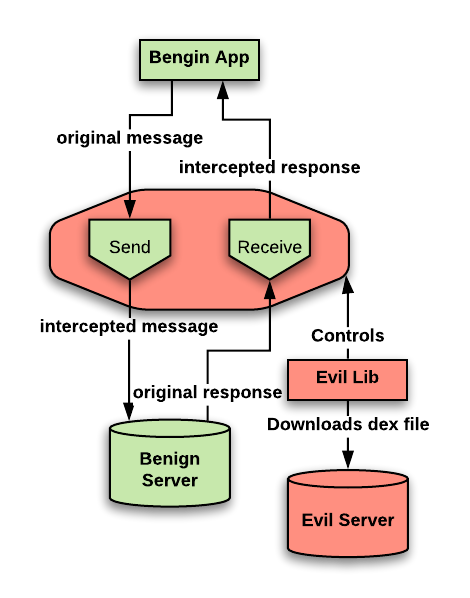
\includegraphics[scale=0.45]{figures/AttackOverview.png}
	\end{center}
	\caption{Attack scenario Overview}
	\label{ModelOverview}
\end{figure}


For the demo app we implemented a simple text messenger: The user can write text messages to a remote server. When the message is sent, the app connects itself to a remote server and establishes an encrypted communication channel using asymmetric cryptography. The server than responds what he has received from the client.

We now act on the attacker's view: The goal is to monitor the communication between the client (benign app) and the remote server. 
Cracking the asymmetric encryption directly isn't a feasible option. We rather want to intercept function calls that handle the sending and receiving of messages before they are encrypted resp. after they are decrypted.


The key component for our attack scenario here is \emph{function hooking}.
From native code we get the ArtMethod objects from the send and receive java methods and redirect them to a native code function. That reads the messages and will change them. This way the user gets notified that the attack is successful. 

As the native hook functions want to call the original functions, we need to do backups. We follow here the way of the YAHFA library and use other java methods to store the original method content. These backup java methods get loaded at runtime: At first, a dex file containing the methods is downloaded from a second (evil) server. And then the dex file are loaded by using the DexClassLoader \footnote{\url{https://developer.android.com/reference/dalvik/system/DexClassLoader.html}}
class.

%Using C++ we can create machine code using some assembly and converting that to bytes.
%Of course the created code has to be made executable. But this is no problem (e.g. through using the Linux functions \emph{mmap}\footnote{\url{http://man7.org/linux/man-pages/man2/mmap.2.html}} or \emph{mprotect}\footnote{\url{http://man7.org/linux/man-pages/man2/mprotect.2.html}} function)).

%Till now we have a foundation to modify machine code (\emph{not} Java Byte Code!). So the next step is to get the function in memory. Fortunately, here helps JNI as it allows to get a class instance with a function call of  \emph{FindClass}\footnote{\url{https://docs.oracle.com/javase/8/docs/technotes/guides/jni/spec/functions.html\#FindClass}} and \emph{GetMethodID}\footnote{\url{https://docs.oracle.com/javase/8/docs/technotes/guides/jni/spec/functions.html\#GetMethodID}} for retrieving a jmethod from a method by its name.

%With the method id we can leverage some runtime information to get access to the compiled machine code. If this is achieved we can change and thus intercept any function from the target app, we like.



\subsection{Implementation}

The memory layout of an ArtMethod is dependent on the specific Android version and the used machine architecture. We also had to write machine code to reset the hotness counter for the backup method. Therefore we constrained ourselves to a specific Android version and one specific machine instruction set. As the instruction set we  chose \emph{i386 (x86)} and 
we chose \emph{Android 8.0 (Oreo)} as the target platform.
Though \emph{arm} is oftener used than \emph{i386}, we preferred \emph{i386}. As for the relative new \emph{Android 8.0 (Oreo)} there weren't any hardware accelerated Android Virtual Device (hAVD) images available for \emph{arm}. Using a hAVD facilitates app development considerably as they perform much faster. 

But there should be mentioned that the attack could also be done for other machine instruction sets and other Android versions, that are using ART (so since Android 5.0). The android version can be examined by the global java constant \emph{android.os.Build.VERSION.SDK\_INT} with JNI.
The differences for the machine instruction set and architecture can be solved on compile time of the native library: In Android Studio the library is compiled for each supported instruction set and architecture. ART loads then at runtime the appropriate library.

To encrypt the communication, we used the TLSv1.2 protocol. 

In order to access the ArtMethod objects of a java method we used JNI, since it allows to get a class instance with a function call of  \emph{FindClass}\footnote{\url{https://docs.oracle.com/javase/8/docs/technotes/guides/jni/spec/functions.html\#FindClass}} and \emph{GetMethodID}\footnote{\url{https://docs.oracle.com/javase/8/docs/technotes/guides/jni/spec/functions.html\#GetMethodID}} for retrieving a \emph{jmethod} from a method by its name. The \emph{jmethod} is actually defined as an empty struct. But it is a placeholder type for not revealing JVM internals to user code. And in fact, the returned \emph{jmethod} object is actually a pointer to an ArtMethod object. At least, this applies for the android platform.


As we want to redirect execution flow to a native function, it would be good to change the original ArtMethod to a native ArtMethod that calls the native function. In theory it should be possible, but we didn't get it running, properly. Although it was possible to call the native function, inside the native function we couldn't call the backup ArtMethod anymore: The execution flow hangs up. Obviously, we forget something to do really that is important, but we didn't find out the solution. 

But we found a workaround, that is stable: Instead of jumping directly to native code, we redirect the execution flow from the original ArtMethod to helper (native) ArtMethod. The helper ArtMethod than is changed so that it directs to the wished native function.

So, our final hooking process as it is done by our attack is illustrated in figure \ref{HookProcess}:

\begin{figure}[H]
	\begin{center}
		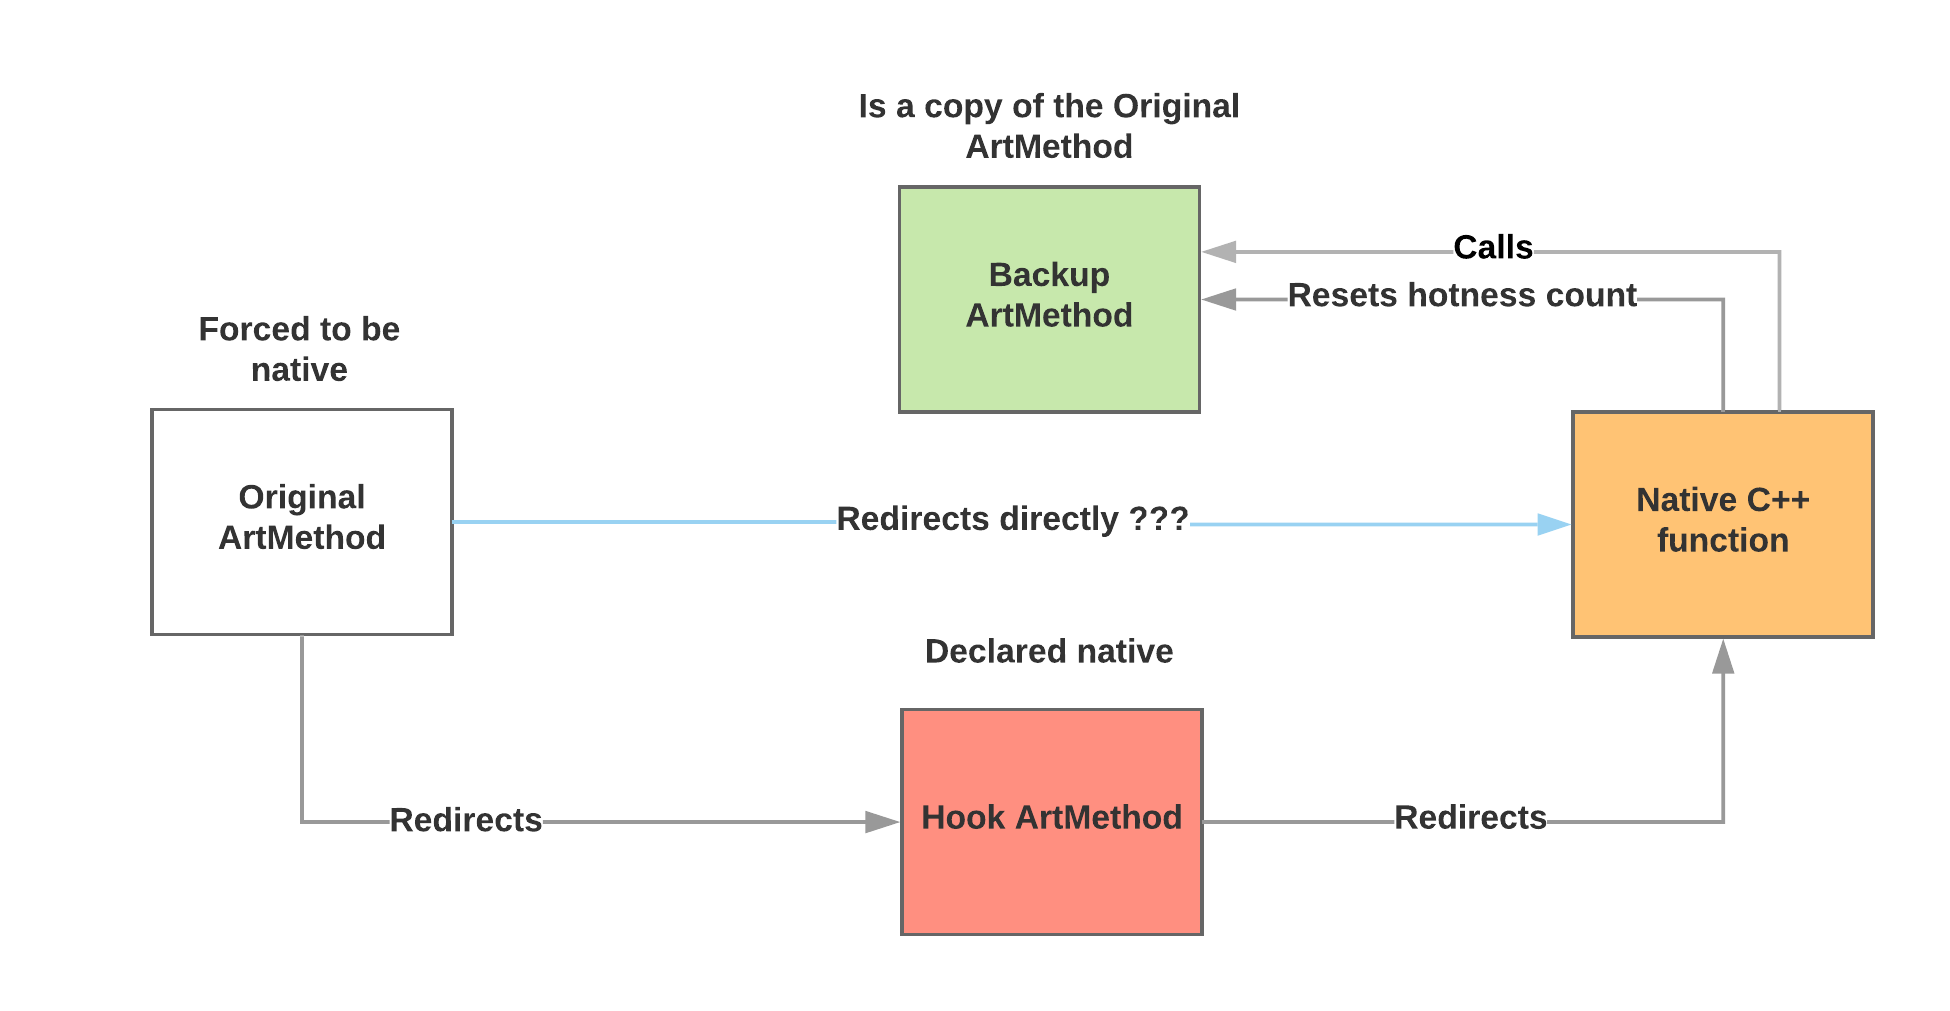
\includegraphics[scale=0.45]{figures/HookProcess.png}
	\end{center}
	\caption{Final hooking process using the hook helper workaround}
	\label{HookProcess}
\end{figure}

%Until now only a proof of concept implementation is done that is rather rudimentary. 
%Besides feature completion the final implementation will be furnished with a nice logging Activity and fully documented source code. 

%The code could be implemented entirely in C++, but it would be (unnecessarily) labor intensive as one has to have deep knowledge of the internals of ART. But it would also be very fragile, since the internals of ART would have to be re-implemented. The behavior is therefore not only dependent from  the machine instruction set, but also from the concrete implementation of interfaces and private functions, that could change from commit to commit.
%This are the reasons to favor a not entirely in C++ code written attack, but instead also use Java code, that cooperates with the native code.

%But there are also some disadvantages of loading additional Java code at runtime: Read and Write Permission for external Storage in the Android app manifest. 

 %To avoid this, an attacker could compile a function to native code and than extract the compiled malicious code and integrate it in the source code as a char array. Then the attacker just needs to make the code executable (e.g. using the \textit{mprotect}. This executable code can then act as replacement hook for any function that has the same method signature (arguments and return value).
% This way, an attacker could entirely use native code for the attack and he/she further needs no additional permissions.
%\subsection{Evaluation}
\section{Conclusion}

In this paper we have shown how JNI could be abused when untrusted native code is loaded by a java android app. Additionally we have illustrated how traditional function hooking can be translated to the ART environment. We used trampoline hooks to intercept messages that were sent or received by the benign app.

For the attack the benign app has to have internet permission \footnote{\url{https://developer.android.com/reference/android/Manifest.permission.html\#INTERNET}}. For our demo app this is no problem, as the benign app itself accesses the internet. But the files that are downloaded from the evil server could also be stored as a char array inside the evil library. So the presented attack actually needs no special permissions.

We didn't find out, why it isn't possible to directly redirect execution flow from an ArtMethod to a native function if the ArtMethod wasn't an ArtMethod for a native java method. But it was possible by a native helper ArtMethod. In future work the reasons for this issue could be find out and properly solved. 